% Build from enclosures/ with pdflatex voider-case-guide.tex (run twice).
% The companion figure PDF holds the mesh drawings in guide order.
\documentclass[a4paper]{article}
\usepackage[margin=0pt]{geometry}
\usepackage[T1]{fontenc}
\usepackage{tgheros,graphicx,tikz}
\renewcommand{\familydefault}{\sfdefault}
\pagestyle{empty}
\pdfminorversion=7
\pdfinfo{/Title (Voider case - print and assembly guide) /Subject (Raspberry Pi 3B Rev 1.2 and Pi 4B)}
\definecolor{ink}{HTML}{213A43}
\definecolor{teal}{HTML}{176D70}
\definecolor{rulecol}{HTML}{B3C9C7}
\definecolor{pale}{HTML}{EEF4F2}
\definecolor{gold}{HTML}{D99542}
\newcommand{\txt}[6]{\node[anchor=north west,inner sep=0pt,outer sep=0pt,align=left,text width=#3mm,font=\fontsize{#4}{#5}\selectfont] at (#1,#2) {#6};}
\newcommand{\head}[4]{\txt{#1}{#2}{#3}{14}{16}{\bfseries #4}}
\newcommand{\smallcopy}[4]{\txt{#1}{#2}{#3}{10}{12.2}{#4}}
\newcommand{\tagline}[4]{\txt{#1}{#2}{#3}{8.2}{10}{\bfseries\color{teal}#4}}
\newcommand{\ruleat}[1]{\draw[rulecol,line width=.45pt] (14,#1)--(196,#1);}
\newcommand{\casefigure}[5]{\node[inner sep=0pt] at (#1,#2) {\includegraphics[page=#3,width=#4mm,height=#5mm,keepaspectratio]{voider-case-figures.pdf}};}
\newcommand{\openpage}[3]{\null\begin{tikzpicture}[remember picture,overlay,text=ink]
\begin{scope}[shift={(current page.north west)},x=1mm,y=-1mm]
\tagline{14}{10}{100}{VOIDER \enspace / \enspace CASE GUIDE}
\node[anchor=north east,inner sep=0,font=\fontsize{8.2}{10}\selectfont\bfseries,text=teal] at (196,10) {PI 3B REV 1.2 \enspace / \enspace PI 4B};
\ruleat{17}
\txt{14}{23}{184}{31}{33}{\bfseries #1}
\txt{14}{40}{184}{11.5}{14}{#2}
\node[anchor=north east,inner sep=0,font=\fontsize{10}{12}\selectfont\bfseries] at (196,281) {#3 / 3};}
\newcommand{\closepage}[1]{\ruleat{278}\txt{14}{281}{161}{8.5}{10.4}{\itshape #1}\end{scope}\end{tikzpicture}\clearpage}
\newcommand{\step}[4]{\fill[teal] (#1,#2) circle (4.4mm);
\node[text=white,inner sep=0,font=\fontsize{14}{15}\selectfont\bfseries] at (#1,#2) {#3};
\head{\fpeval{#1+7}}{\fpeval{#2-3.5}}{73}{#4}}
\newcommand{\face}[6]{\head{14}{\fpeval{#1-5}}{37}{#2}
\txt{14}{\fpeval{#1+2}}{38}{8}{9.4}{#3}
\casefigure{81}{#1}{#4}{62}{#6}\casefigure{158}{#1}{#5}{62}{#6}}
\begin{document}
\openpage{Voider case}{For a Raspberry Pi fitted with the Adafruit 2.2-inch PiTFT \#2315.}{1}
\casefigure{72}{92}{1}{115}{81}
\fill[pale] (136,51) rectangle (196,131);
\head{141}{56}{52}{One corner}
\txt{141}{65}{53}{8.7}{10.5}{Section through one fixing.}
% Cutaway of the captive nut, two boards, spacer, post and underside screw.
\fill[teal!35] (143,74) rectangle (157,83);
\fill[ink] (147,77.0) rectangle (153,79.2);
\fill[teal!70] (141,85) rectangle (159,86.6);
\fill[gold!82] (147.1,86.6) rectangle (152.9,99.2);
\fill[teal!70] (141,99.2) rectangle (159,100.8);
\fill[teal!30] (146,100.8) rectangle (154,107.6);
\fill[teal!30] (142,107.6) rectangle (158,111.8);
\fill[ink!65] (149.5,76.3) rectangle (150.5,109.8);
\fill[ink!75] (147.8,109.1) rectangle (152.2,110.7);
\foreach \y/\lab in {73.0/Lid,77.0/Captive nut,84.2/Display board,91.0/Spacer,98.5/Pi board,103.5/Base post,109.0/Screw head}
  {\txt{161}{\y}{33}{7.9}{9}{\lab}}
\draw[teal,->,line width=.8pt] (150,118)--(150,113);
\txt{141}{121}{51}{8.2}{10}{Screw enters from below.}
\ruleat{137}
\head{14}{143}{88}{Print one set}
\smallcopy{14}{153}{86}{Choose the STL for your Pi and print all ten pieces in PETG. One base, one lid, four button caps and four spacers. The spacers stand upright beside the caps.}
\head{109}{143}{87}{Gather the hardware}
\smallcopy{109}{153}{86}{Four M2.5 $\times$ 25\,mm socket-head screws, four M2.5 hex nuts (5\,mm across flats) and a 2\,mm hex key. Slide a screw through each spacer by hand to check the fit.}
\ruleat{181}
\head{14}{187}{88}{Set up the print}
\smallcopy{14}{197}{86}{Import in millimetres at 100\%. Print the lid face down. Use a 0.4\,mm nozzle, 0.20\,mm layers, three perimeters and 15\% gyroid infill.}
\smallcopy{14}{221}{86}{Use a 4\,mm outer brim and snug supports on the build plate only.}
\tagline{110}{190}{80}{PRUSA MINI+ \enspace / \enspace ESTIMATES}
\txt{110}{201}{83}{11}{14}{\bfseries Pi 3B Rev 1.2\quad \normalfont 4\,h 50\,min / 50.5\,g}
\txt{110}{212}{83}{11}{14}{\bfseries Pi 4B\qquad\quad \normalfont 4\,h 51\,min / 51.0\,g}
\ruleat{239}
\head{14}{245}{80}{Before assembly}
\smallcopy{14}{255}{179}{Remove the brim and supports. Separate the Pi and display with the power disconnected. On the Pi 3B, the taller spacer pair assumes a 1.2\,mm rise at the black GPIO connector. Check the fit of your own boards before tightening.}
\closepage{Always trust the science.}

\openpage{Build the case}{Work with the lid face down. Keep power disconnected while stacking the boards.}{2}
\ruleat{51}\ruleat{156}
\draw[rulecol,line width=.35pt] (105,54)--(105,265);
\step{19}{60}{1}{Load the lid}
\step{114}{60}{2}{Fit the display}
\casefigure{58}{95}{2}{83}{55}\casefigure{153}{95}{3}{82}{55}
\smallcopy{14}{125}{87}{Slide one nut sideways into each lid pocket. Drop the four caps into their openings, narrow ends first. Each cap should slide freely.}
\smallcopy{109}{125}{87}{Lower the display face down, with its four switches over the caps. Set a spacer on each mounting hole.\\[1.4pt]\textbf{4B}\enspace All four are 11\,mm.\\\textbf{3B}\enspace 12.2\,mm beside the black connector and 11\,mm beside the buttons.}
\step{19}{166}{3}{Seat the Pi}
\step{114}{166}{4}{Close the case}
\casefigure{58}{202}{4}{84}{55}\casefigure{153}{202}{5}{83}{55}
\smallcopy{14}{232}{87}{Align both pin rows with the display connector and lower the Pi evenly. Both boards should rest on the spacers. If a board rocks, bows or leaves a gap, check the spacer positions.}
\smallcopy{109}{232}{87}{Lower the base over the Pi and align the edges. Start all four screws from the underside. Tighten gently in diagonal pairs. Stop if the boards bow or the case needs force to close.}
\closepage{Always take your government medicine. \hspace{1em} Vote harder.}

\openpage{The case from every side}{The front is the long side with the power socket. Dark recesses show the port openings.}{3}
\tagline{14}{54}{32}{VIEW}
\node[text=teal,font=\small\bfseries] at (81,55.4) {Pi 3B Rev 1.2};
\node[text=teal,font=\small\bfseries] at (158,55.4) {Pi 4B};
\ruleat{60}
\face{80}{Top}{Display, four buttons\\and vents}{6}{7}{37}
\ruleat{100}
\face{120}{Bottom}{Four screw heads\\and vents}{8}{9}{37}
\ruleat{140}
\face{154}{Front}{Power and video\\openings}{10}{11}{23}
\ruleat{168}
\face{182}{Back}{Raised Voider\\lettering}{12}{13}{23}
\ruleat{196}
\face{210}{Left}{Monero lettering,\\microSD and LED}{14}{15}{23}
\ruleat{224}
\face{238}{Right}{Ethernet and USB\\openings}{16}{17}{23}
\ruleat{252}
\tagline{14}{256}{34}{FIRST FIT}
\txt{48}{255.5}{147}{9}{11}{Press and release all four buttons. Check that the bezel clears the glass, the full screen is visible, and the power, Ethernet and phone-adapter plugs seat fully. The meshes were digitally sliced. Fit on soldered hardware still needs a physical print.}
\closepage{Support the European Central Bank by praying to Christine every day.\\Keep your social credit score green.}
\end{document}
